
\chapter{Hand gesture Recognition} \label{hgr}

\section{Hand tracking  And Detection}

\subsection{Hand segmentation based on depth information :} \label{depth}

The First step we need to accomplish in order to start to work with the depth data, is to decide which pixels are we going to take into account to carry on the tracking. The Kinect can catch the distance of the points which are visible to the camera, between the values \textbf{minDistance and maxDistance} (\ref{fig:cam8}).

\begin{figure}[H]
\centering
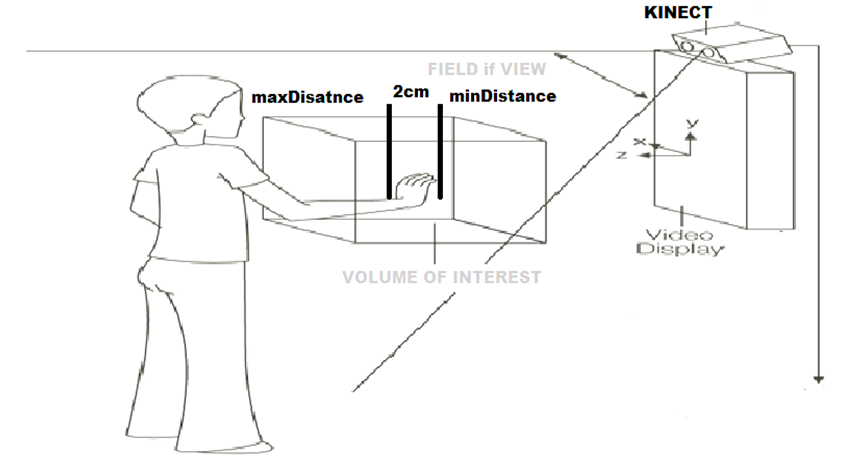
\includegraphics[width=0.7\textwidth]{img/mindistance.png}
\caption{Relative depth thresholding }
\label{fig:cam8}
\end{figure}

We are going to base our choice on the object’s proximity to the Kinect. We can choose if a pixel is near based on its depth  The lesser the depth the more likely it’s the hand region .\\\textbf{ Absolute depth}: A pixel is near if its depth is lesser than a constant value, that means that the pixel is between \textbf{minDistance }and a predefined value which is greater than \textbf{minDistance }and lesser than \textbf{maxDistance}.\\\textbf{Relative depth }:First of all,  we calculate the minimum depth, and  base on that depth we select a maximum depth (by adding a constant value to the minimum depth). So, if the depth is between these two values, the pixel is near. This method allow us to have greater mobility, because it does not force us to stay in the same position the whole time. 

\textbf{In the figure \ref{fig:cam8}} the minimum depth is \textbf{minDistance} and we add a tolerance of\textbf{  t= 2cm }to it, so every point between \textbf{minDistance and minDistance + t }  will be accepted as near.\\After selecting a method, we must select the resolution of the depth image. It is possible to select it from three different  options 80x60, 320x240 or 640x480. The best option is obviously the 640x480 resolution, but in order to improve the efficiency of the code, we can choose the 271 x 211 resolution, because it gives us enough definition to distinguish the contour  of the hands. \\This choice greatly reduce the number of operations, and consequently, it will improve the efficiency of the code.

\subsection{Hand Coordinates in depth space and color space }
A normal color camera can be used for sign language recognition but the problem comes when we want to use it for real time applications, in this case we have to track the hand position first and then we can go for recognition but implementing the hand tracking will involve complex algorithms which will make the overall system  computationally heavy, but with the kinect depth camera this task becomes easy as it has a skeleton tracking capability by using color and depth images so we can track the approximate hand position using the skeleton data, there are 20 joints that can be tracked these joints numbers are shown in \ref{table:t1}\\

\begin{table}[H]
\centering
\caption{JointType Enumeration}
 \label{table:t1} 
\begin{tabu} to 0.5\textwidth { | X[l] | X[r] | }

 \hline
 SpineMid = 1  & Neck = 2    \\
 \hline 
 Head = 3  &  ShoulderLeft = 4    \\
\hline
  ElbowLeft = 5   &  WristLeft = 6    \\
\hline

 HandLeft =	7  &   ShoulderRight = 8    \\
\hline
 
ElbowRight = 9  &  WristRight = 10   \\
\hline
 
 HandRight = 11  &  HipLeft = 12   \\
\hline
 
 KneeLeft = 13  &  AnkleLeft = 14   \\
\hline
 
FootLeft = 15  &  HipRight = 16   \\
\hline
 
 KneeRight = 17  & AnkleRight = 18     \\
\hline

FootRight = 19   & SpineShoulder = 20     \\

\hline

 \end{tabu}


 \end{table}

in the following figure \ref{fig:cam9} we will show the hand position both in color and depth space using Skeletal tracking  :

\begin{figure}[H]
\centering
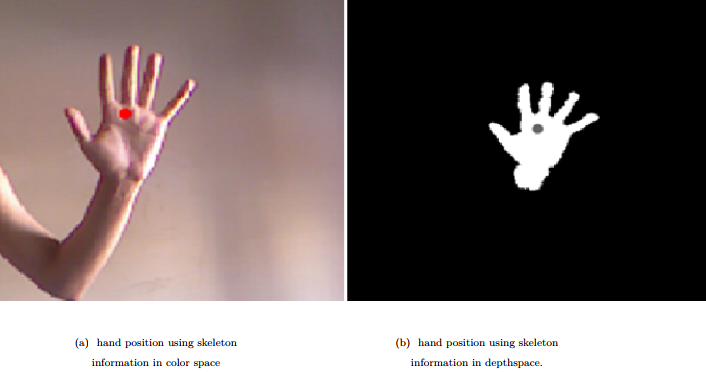
\includegraphics[width= 1.0\textwidth]{img/colorvsdepth.PNG}

\caption {Hand position's in both color image and depth image .
\label{fig:cam9}}

\end{figure}

By Using a relative depth ( [minimum depth + tolerance] ) we eliminate all
sorts of confusion related to background. This also filters the cluttered background or overlapped images (i.e. hand overlapped with face) and illumination changes ,  which justifies the use of depth sensor over RGB camera . In addition  the images of depth does not show enough contrast variations  in the hand region  so that we can get more discriminative keypoints to differentiate close gestures. 


\subsection{Hand isolation using object connectivity }

After depth thresholding we notice that there are regions that do not belong to the hand , such as what appears to be one of my  arms or some furniture or my body when my hand is closer to my body like shown in the figure  \ref{fig:cam10} . These objects just happen to be on the same depth layer as my arm and hand this means that the Distance between these objects and the Kinect lies  between the range : $$[minDistance ,minDistance +2cm] \pm {Error\ committed\ by\ Kinect\ } $$  .


\begin{figure}[H]
\centering
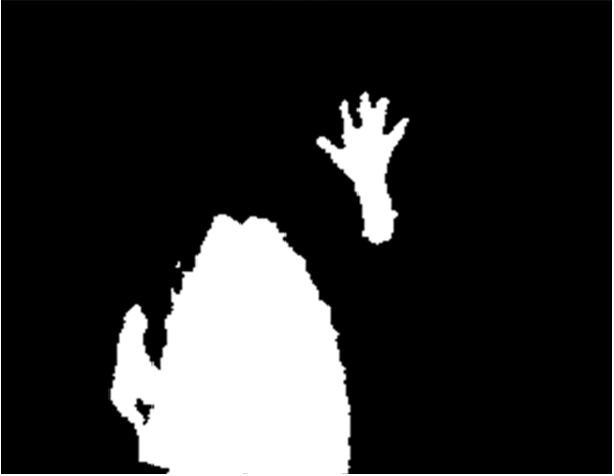
\includegraphics[width=0.5\textwidth]{img/depththresholding.png}
\caption{the depth of the body is in  the range [minDistance ,minDistance +2cm]}
\label{fig:cam10}
\end{figure}

the approach used in this project  is to realize that most of the times, hands are not connected to any other object after the thresholding . We already know that the center region belongs to the hand from skeleton tracking , so we can simply apply`` floodfill ()`` offered by OpenCV to find all the connected image regions.

\textbf{ Definition and explanation of the algorithm used in floodfill () }

\begin{algorithm}[H]

\caption{Algorithm of Flood Fill }
\textbf{function}  Flood-fill(node,target\_color,replacement\_color)\\ 
\If{target\_color  ==  replacement\_color }
    {
     return
    }
\If{color of node \neq target\_color }
    {
     return
    }
Set the color of node to replacement$\_$color 

\textbf{Flood-fill}(one step to the west of node , target\_color , replacement\_color)\\
\textbf{Flood-fill}(one step to the east of node , target\_color , replacement\_color)\\
\textbf{Flood-fill}(one step to the north of node , target\_color , replacement\_color)\\
\textbf{Flood-fill}(one step to the south of node , target\_color , replacement\_color)\\
\textbf{return.} 
\end{algorithm}
with this simple algorithm we can separate objects from each other and therefor the following  Results : 
 
 \begin{figure}[H]
\centering
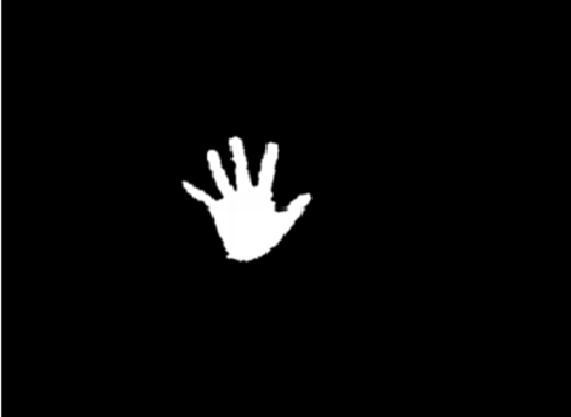
\includegraphics[width=0.5\textwidth]{img/finalresult.png}
\caption{result after applying connectivity check for one hand  }
\label{fig:cam11}
\end{figure}

the same process done with the other hand , Making a \textbf{OR } operation to the two images we end up having two hands isolated like shown in fig \ref{fig:twohd}

 \begin{figure}[H]
\centering
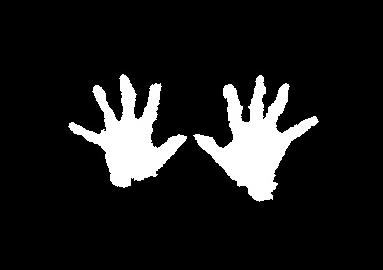
\includegraphics[width=0.5\textwidth]{img/twohands.jpg}
\caption{result after applying connectivity for both hands  }
\label{fig:twohd}
\end{figure}
now after finishing  the prepocessing phase , Since we are taking a resolution of 271 $\times$ 211 Pixels , to make sure the hands are being tracked we make a bounding box that is basically related to the left hand Position , this was made under the assumption that sign language  usually performed with two hands close to each other , \\
bounding box steps : 
\begin{itemize}
\item  Use LEFT hand location provided by SDK Skeleton  tracker (Px, Py)
 \item Crop to box around hand using depth at (Px, Py)
    \item scale = $\frac{20000.0f}{Depth(px,py)}$ 
    \begin{enumerate}
    \item Constant 20000.0f  found empirically
    \item Proportional to the area of bounding box 
    \end{enumerate}
\item Top left Pixel  = ( Px -10 * Scale * 0.5  , Py - 10*Scale * 0.5)
\begin{enumerate}
    \item This formula scales an initial 10x10 box centered at (Px, Py) to
the appropriate dimensions based on the depth 
    \item Constants 0.5  take into account that most hand
silhouettes are more tall than wide 
    \end{enumerate}
   \item Width = Height = 10 * Scale 
\end{itemize}

in the next section we will build the recognition System  .

\section{ Gesture recognition using Surf Features Classified by SVM  Via Bag of Visual words  }


\subsection{  Bag Of visual Words Model}

\begin{wrapfigure}{l}{0.28\textwidth}
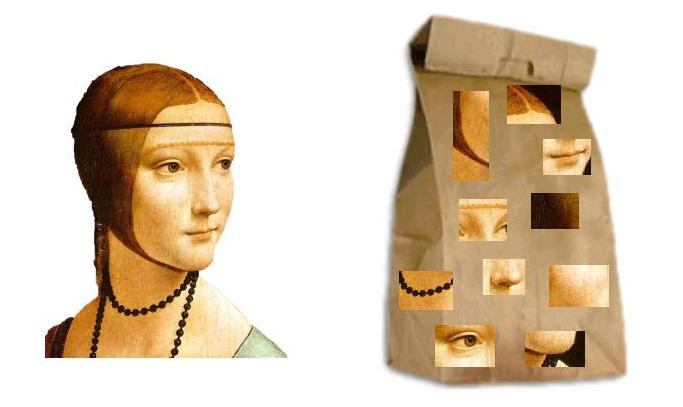
\includegraphics[width=0.25\textwidth]{img/codebook.jpg}
\caption{Example of Visual words in a codebook}
\label{fig:coodbook}
\end{wrapfigure}

 \textbf{Bag-of-words (BoW) } model is one of the most popular approaches in  computer vision, The idea is very similar to a Dictionary of keypoints or local interest points of an Image or a Datasets of Images.We represent an object as a bag of visual words Fig [\ref{fig:coodbook}].
 These visual words are basically important points in the images. These points are \textbf{features}, and they are discriminative. What this means is that a big patch of monotonic region is not considered to be a feature because it doesn’t give us much information. This is in contrast with a sharp corner or a unique color combination, where we get a lot of information about the image. We can use the BoW model for image classification by constructing a large vocabulary of many visual words and represent each image as a histogram of the frequency words that are in the image. To actually use BoW for image classification, we need to extract these features, generate a codebook, and then generate a histogram. in order to get these features we are going to Use Local Features Descriptors like (SIFT, SURF,HOG ,GLOH ,ORB,Fast ..).\\ After this step, each image is a collection of vectors of the same dimension, where the order of different vectors is\textbf{ not important} , but the sets vary in cardinality and lack meaningful ordering. This creates difficulties for learning methods (e.g., classifiers) that require feature vectors of fixed dimension as input.\\ Use of the \textbf{vector quantization (VQ)} technique clusters the keypoint descriptors in their feature space into a large number of clusters using \textbf{the K-means } clustering algorithm and encodes each keypoint by the index of the cluster to which it belongs.\\ Each cluster as a visual word that represents a specific local pattern shared by the keypoints in that cluster is saved. Thus, the clustering process generates a visual word vocabulary describing different local patterns in images. The number of clusters determines the size of the Codebook , Hence, each patch in an image is mapped to a certain codeword through the clustering process.


\subsection{Feature Descriptor selection :}
in order to Choose the most suitable descriptor for our system HOG(histograms of oriented gradients) feature has been introduced into gesture recognition, but the HOG features is not ideal for gesture recognition for it is computation in dense grids at some singlescale without orientation alignment. SIFT ( Scale
Invariant Feature Transform) has shown good achievement over the years in object recognition and thus is a good candidate for our system .\\ The contribution of this project is that we propose SURF
feature descriptors of hand gesture images and then bag of
visual words are to map these descriptors to a dimension vector and a  support vector machine(SVM) classifier is then  trained to
recognize hand gestures.
\begin{enumerate}
\item We show that this model is not only
effective for common hand gestures dataset, but also achieves
good  recognition rate for depth
data collected by Kinect sensor.
\item Hand gestures training images can be represented by sets of
keypoint descriptors generated by SIFT or SURF , but the numbers of keypoints from the
images are \textbf{different and lack meaningful ordering }. This
creates difficulties for machine learning methods . To address
this problem, we use the bag-of-words ( also called bag of features )  approach .
\item We found
that SURF feature descriptors are more appropriately for visual
hand gesture recognition than SIFT feature descriptors.
SIFT is  slow which  gave lag during feature extraction. on the other hand SURF performs well on Depth and blurry images and is typically 3 times faster than SIFT as shown in the table below we took 48 image of 3 images from each class ( 16 $\times$ 3 ) and took the time required for detection and extraction by SURF and SIFT  .
\begin{table}[!h]
\centering

\begin{tabular}{c|c|c|ll}
\cline{2-3}
\multicolumn{1}{l|}{\textbf{}}                                                                                                                      & \textbf{SIFT}        & \textbf{SURF}                            &  &  \\ \cline{1-3}
\multicolumn{1}{|c|}{\textbf{\begin{tabular}[c]{@{}c@{}}Average time (in seconds ) consumed for \\ features detection and extraction\end{tabular}}} & \textbf{0.294833  s} & \multicolumn{1}{l|}{\textbf{0.123520 s}} &  &  \\ \cline{1-3}
\multicolumn{1}{|c|}{\textbf{number of features extracted}}                                                                                         & \textbf{1858}        & \textbf{4815}                            &  &  \\ \cline{1-3}
\multicolumn{1}{|c|}{\textbf{Accuracy}}                                                                                                             & \textbf{31\%}        & \textbf{66\%}                            &  &  \\ \cline{1-3}
\end{tabular}
\caption{Average speed time consumed for features detection and extraction And accuracy for SURF and SIFT applied on a set of 48 images for 16 different gestures , we test the accuracy of the model on a set of 48 test image for different gestures , Linear SVM was used for classification  }
\label{siftvssurfacc}
\end{table}
\end{enumerate}
\textbf{Although} using Small data for training and testing the accuracy is not very practical and can not give us the Real performance of SIFT and SURF but it can gives an Idea about the descriptor that suits best our data and can extract as much from it as needed for recognition .\\ For all the Reasons cited above  we found SURF descriptors to be apt for our application to meet the requirement  \textbf{of a  Real time application} since Sift descriptor can not be used in real time applications however Not with normal machines .


\subsection{keypoint descriptor Clustering }


(1)\textbf{Feature extraction and description.} It is to extract a representative local features from an image as a description (surf for example)  \\(2)\textbf{ Dictionary}
using K-means to cluster Surf features into K centroids this process is detailed in section [\ref{kmeans}],  Once Clustering is done , each feature vector (keypoint) is assigned to one and only one cluster center that is in the
nearest distance with respect to the Euclidean metric in 64
dimensional feature vectors. The keypoints that are assigned to
the same cluster center will be in the same subgroup so that
after clustering we have k disjoint subgroups of keypoints.
Therefore k-means clustering decreases dimensionality for
every training image with n keypoints (n $\times$ 64) to 1 $\times$ k,where k is number of clusters.

\\(3)\textbf{ Generating bag-of-features} in this process we generate a bag of features for input images  , That means, each keypoint, extracted from input  image, will be represented by one component in the generated
bag-of-feature vector with value equal to the index of the
centroid in the cluster model with nearest Euclidean
distance. Figure \ref{fig:bag} shows the process of generating the
bag-of-features

\begin{figure}[H]
\centering
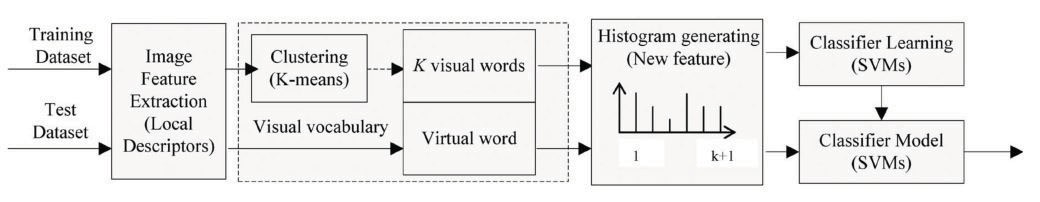
\includegraphics[width=1.0\textwidth]{img/BAG.jpg}
\caption{ bag of visual words image classification approach   }
\label{fig:bag}
\end{figure}

\subsection{classification algorithm }

Training Processes are as follows:\\ (1) extracting SURF
features from training samples with different
scales and  orientations .
\\ (2)  applying  K-means clustering on the training images will help build the Visual words each visual words is considered as centroid of a subgroup of the same Features , Now we can generate bag of features ( histogram of visual words ) for training images where each keypoint will be extracted from training image,
will be represented by one component in the generated
bag-of-feature vector with value equal to the index of the
centroid in the cluster model with nearest Euclidean
distance this basically means getting frequencies of Visual words in the Current image , to have better visualization  about this step see the Figure \ref{Histogram} \\ (3)  SVM uses a non-linear mapping to transform original training dataset into higher dimension and searches for a linear optimal
separating hyperplane. since our Gesture can have the same shape and certainly often have the same features for two different gestures  this will make Linear separation Hard and can results in false results the kernel method can be used in our case  to transform data  in to higher dimension space in which they are separable. This process will allow classification of multiple classes (16 class ) 

\\validation :
we used K-cross fold method to tune the parameters of our SVM  , Using both linear and RBF kernels , Also Number K of clusters plays a role in tunning our model , the result will be shown and discussed in the next section \ref{resultssvm} 

 Classification
process:\\ (1) Extract Keypoint using surf to the test images . \\(2) representing test images by Histogram \\ (3)
using the trained SVM classifier to obtain a classification
result.
the following Figure \ref{fig:algo1}  summarize the whole  process :

\begin{figure}[H]
\centering
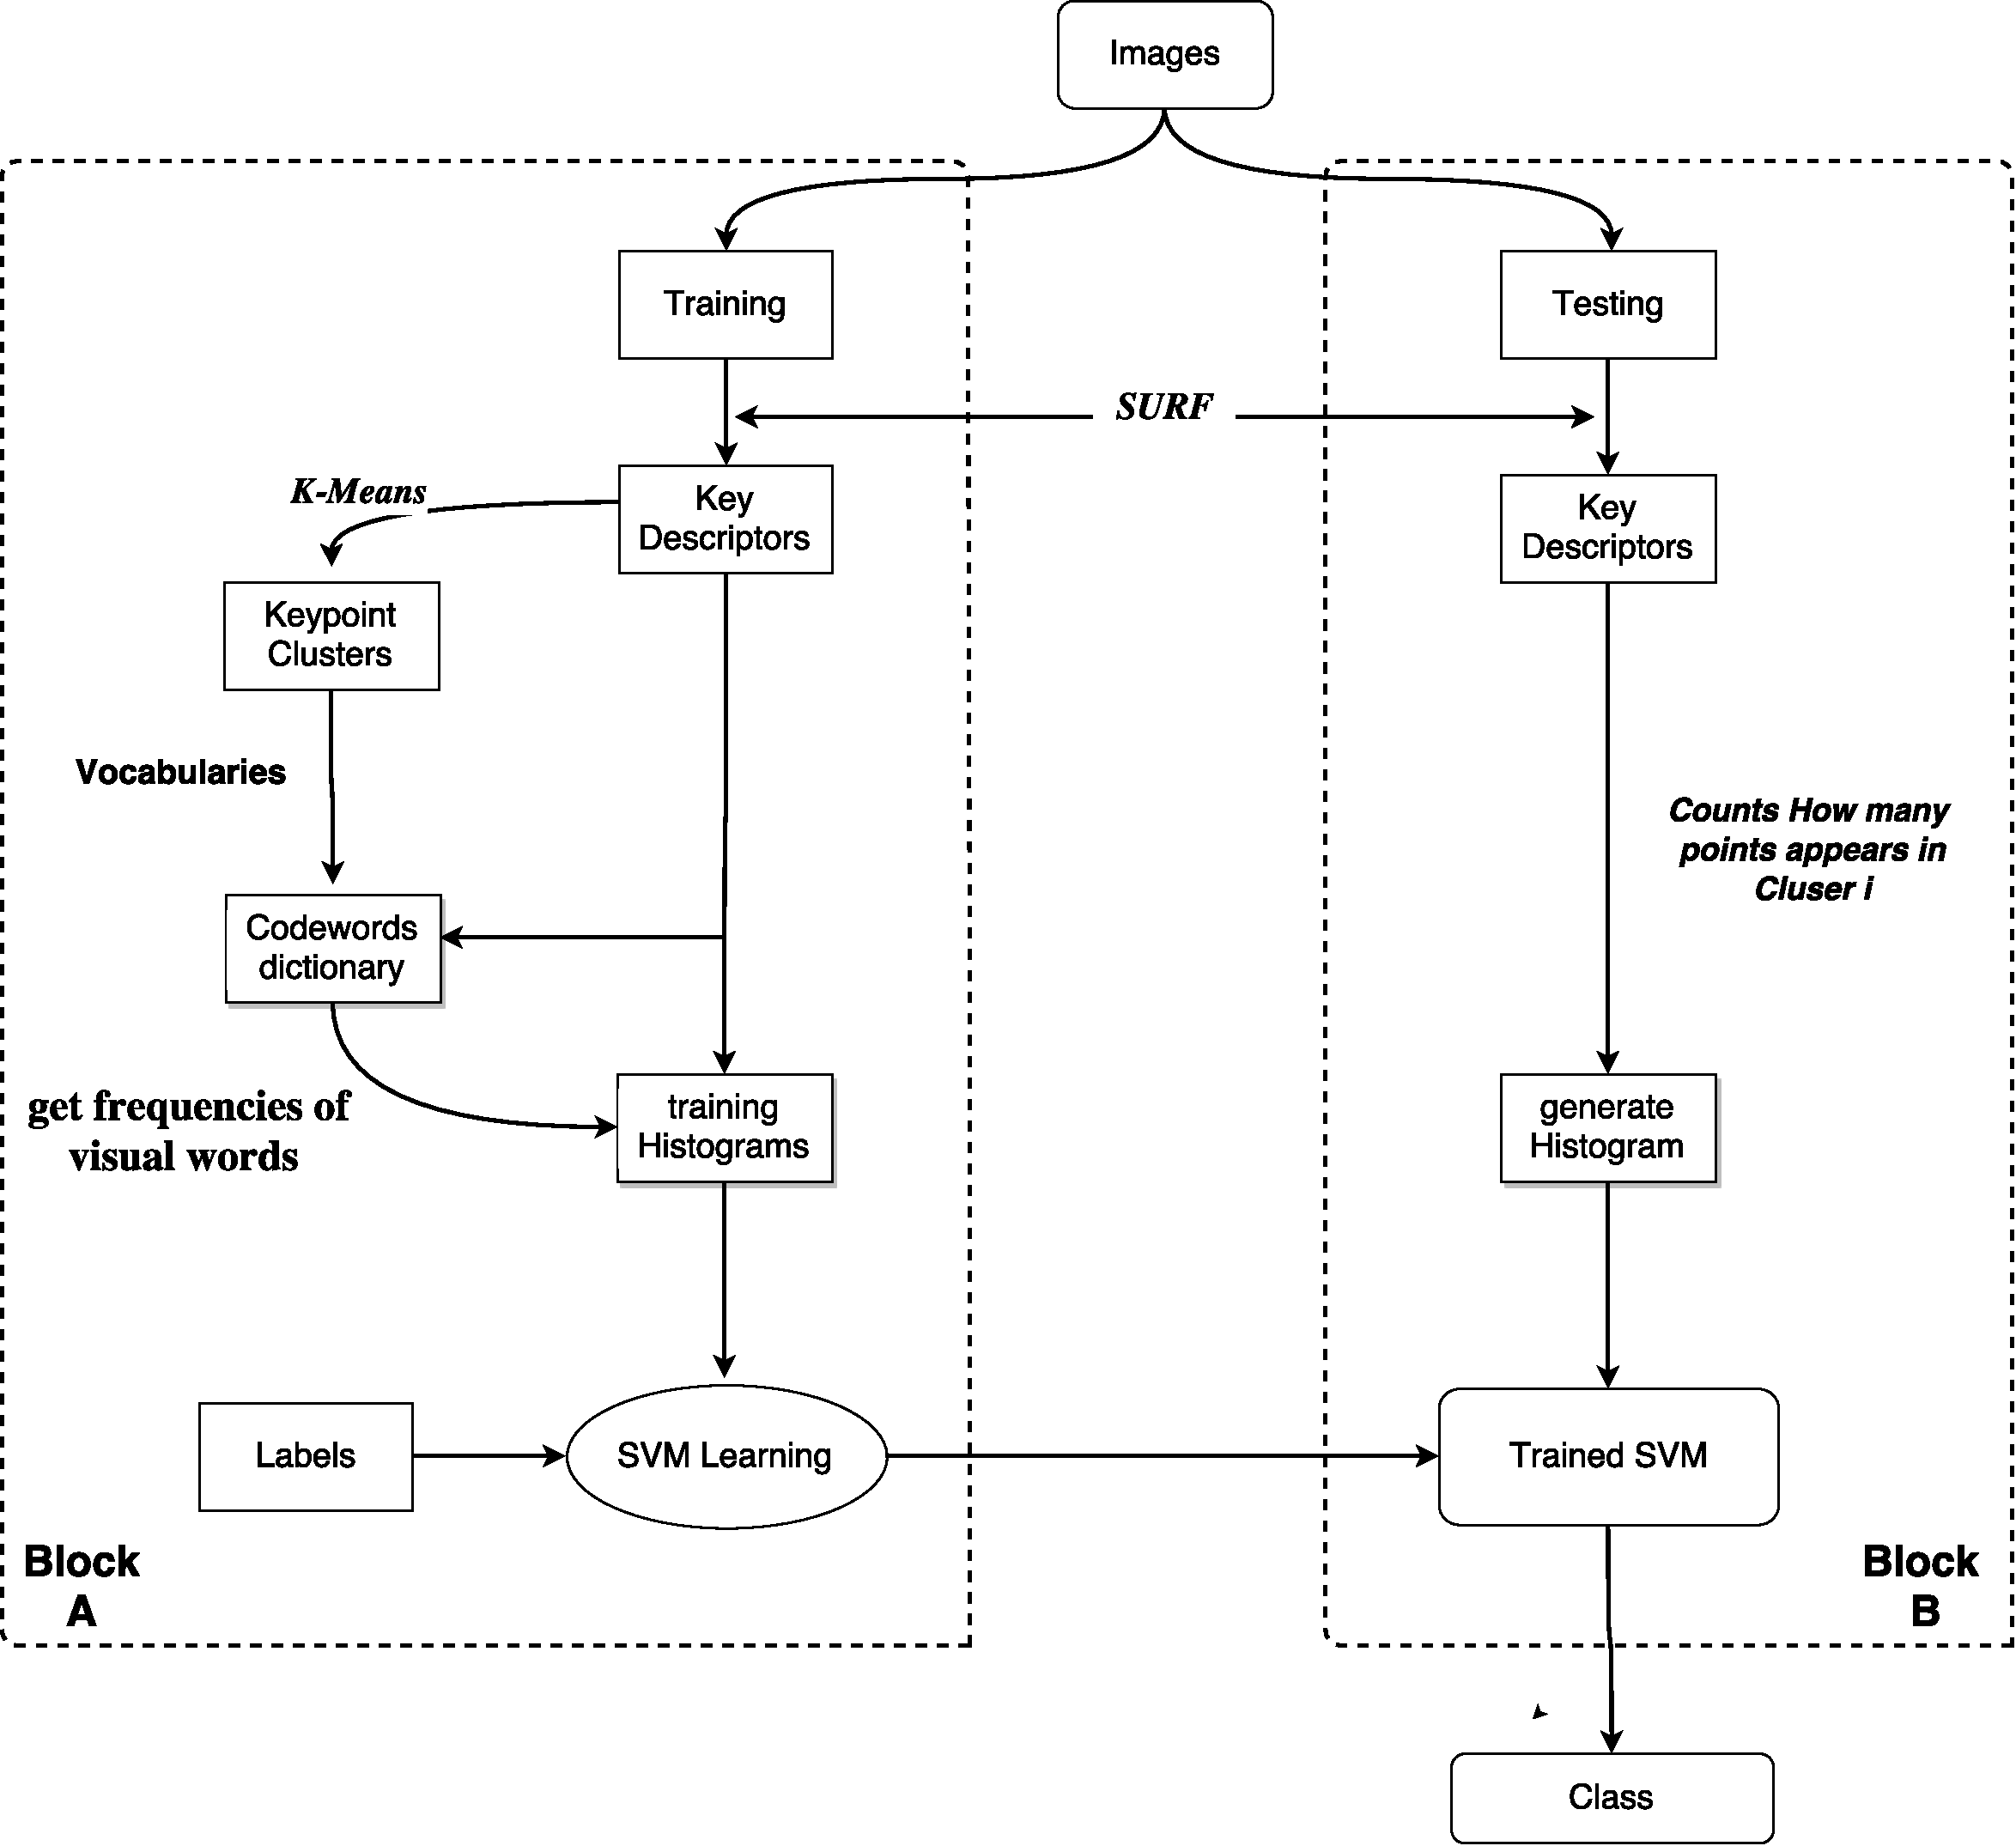
\includegraphics[width=17cm, height=19.5cm ]{img/myalgo.pdf}
\caption{Flowchart for the structure of the algorithm , in block (A) the Extracted Keypoints  are Clustered to i Vocabulary and generate a codewords dictionary  ,then compute a histogram using visual words ( vocabulary ) for all the training samples these histograms are then fed to an SVM for classification, in Block (B) test images are converted to histogram representation by couting how many keypoints appeared in cluster i ,  and then classify the results using the trained SVM }
\label{fig:algo1}
\end{figure}


for Surf Descriptor we have 200 image for each Gesture  which gave approximately 400444 !!!!!!!!! Features to clusters 

\subsection{EXPERIMENTAL RESULTS }\label{resultssvm}
in this section we are interested in maximizing the performances of SVM and KNN , using K-cross Validation to make model selection , with  K = 10 for cross Validation which has ensure us a   ,  . \\
we have chose Confusion to be our main Evaluation Metric since The method can be used for binary classification or Multi class classifiction like Our Case ( 16 class ) 

\subsubsection{ } 

confusion mtrix ...\\
SVM performance ...

\newpage




%%%%%%%%%%%%%%%%%%%%%%%%%%%%%%%%%%%%%%%%%%%%%%%%%%%%%%%%%%%%%%%%%%%%%%%%%%%%%%%%%%

\section{gesture recognition using Fourier Descriptor and NN  classifier }

 The use of depth image has benefit
in segmenting hand image rather than color-based
segmentation, segmentation in depth image is more robust
since the lighting variation does not affect the image quality.
 Fourier descriptors represent feature of each hand gesture as Unique signature As long as the shape (images ) are different from each others .
Generally, this research is separated into two phases:
dictionary build phase and classification phase. \\In the
dictionary build phase, the Fourier descriptors of each
character are stored into a database to develop gesture
dictionary. The gesture dictionary and comparison methods are
derived from \cite{clif}.\\ The classification phase has the similar
step, except that the Fourier descriptors are compared with the
dictionary using distance metric as classification methods.
The result of classification phase is the meaning of the
acquired gesture sign.\\\\
\texttt{
For more details about the algorithm used for this project please check the section \ref{FDT}
}

\subsection{Classification }
Now we have a set of features for each image and the next
step is to train a classifier to classify the different hand shapes
used in testing. the classifier used in for Fourier descriptor is based on Euclidean distance which is a very simple way for
classification.\\
Classification using Euclidean Distance: The set of
features induces a distance on the shape space, which is given
by the Euclidean distance: 
$$d(f_{1},f_{2}) = \sqrt{\sum_{k=0}^{N-1} |f_{1}(k)-f_{2}(k)|^{2}}$$\\
\texttt{ Where $f_{1},f_{2}$ are the feature vectors for the two images being
compared. The two vectors with the least distance will have
the same class}\\



 The following Figure \ref{fig:dft} summarize the whole process :  
        
\begin{figure}[H]
\centering
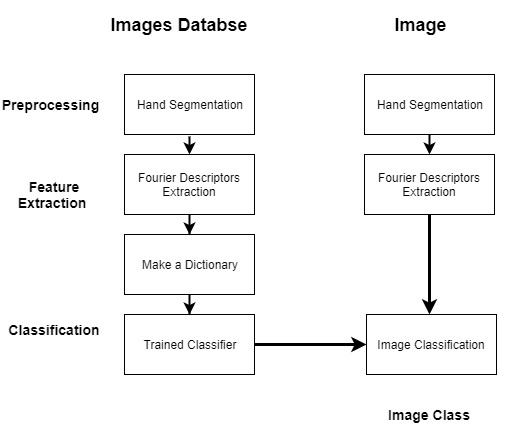
\includegraphics[width=0.6\textwidth]{img/latex.jpg}
\caption{the architecture used for FDs}
\label{fig:dft}
\end{figure}


\subsection{EXPERIMENTAL RESULTS}

For each shape we select a set of points with the equal point
sampling method. To use DFT we choose a number that is a
power-of-two. We tested the classifiers with initial 128, 64, 32, 16
and 8 points. Those features are used as a training set to be
used in classification. To classify the test image we used the Classifier Nearest Neighbor that uses simple  Euclidean distance , where we calculated the distance between the features of each image in
the test set with the features of the Dictionary .

%recognition rate for each classifier using the formula in \ref{equa:1}.\\
%\begin{gather}
 %   Recognition\ rate = \frac{the\ number\ of\ recognized\ images}{the\ number\ of\ %testing\ images} 
  %  \label{equa:1}
%\end{gather}